\documentclass[utf8]{ctexart} %中文文档类
\usepackage[left=2.50cm, right=2.50cm, top=2.50cm, bottom=2.50cm]{geometry} % 页边距
\usepackage{indentfirst} % 首行缩进
\usepackage{fancyhdr} % 设置页眉、页脚
\renewcommand\headrulewidth{0pt}% 页眉与正文之间的水平线粗细
\usepackage{ctexcap} % 标题是中文的
\usepackage{helvet} % 用来指定beamer使用的字体
\usepackage{hyperref} % bookmarks 
\usepackage{multicol} % 分栏

\usepackage{amsmath, amsfonts, amssymb} % 数学公式、符号
\usepackage[english]{babel} % 数学公式标准
\usepackage{bm} % 加粗方程字体 
\usepackage{float}

\usepackage{graphicx} % 图片 
\usepackage{url} % 超链接 

\usepackage{multirow} % 表格
\usepackage{booktabs} % 三线表
\usepackage{longtable} % 长表格

%\usepackage{algorithm} % 算法或伪代码
%\usepackage{algorithmic} % 算法或伪代码
\usepackage[linesnumbered,lined,boxed,commentsnumbered]{algorithm2e}

\usepackage{enumitem} % 枚举环境宏包

%\renewcommand{\algorithmicrequire}{ \textbf{Input:}} 
%\renewcommand{\algorithmicensure}{ \textbf{Initialize:}} 
%\renewcommand{\algorithmicreturn}{ \textbf{Output:}} %算法格式

\newtheorem{theorem}{\indent 定理}[section]
\newtheorem{lemma}[theorem]{\indent 引理}
\newtheorem{proposition}[theorem]{\indent 命题}
\newtheorem{corollary}[theorem]{\indent 推论}
\newtheorem{definition}{\indent 定义}[section]
\newtheorem{example}{\indent 例}[section]
\newtheorem{remark}{\indent 注}[section]
\newenvironment{solution}{\begin{proof}[\indent\bf 解]}{\end{proof}}
\renewcommand{\proofname}{\indent\bf 证明}

\pagestyle{fancy} \lhead{} \chead{} \lfoot{} \cfoot{} \rfoot{}
\pagestyle{plain}
\hypersetup{colorlinks, bookmarks, unicode} % unicode 
 
\title{\textbf{Euler B\`{e}zier 曲线与Euler B样条曲线}}
\author{\bf 王庶霖}
\date{}

\hypersetup{
colorlinks=true,
linkcolor=black
} % 使目录为黑色字
\begin{document}  
		\maketitle
		\renewcommand{\contentsname}{目录} 
		\tableofcontents
		\newpage 
		\renewcommand{\abstractname}{\Large 摘要}

		\begin{abstract}
		\addcontentsline{toc}{section}{摘要}
		\normalsize
		这里是摘要内容。这里是摘要内容。这里是摘要内容。这里是摘要内容。这里是摘要内容。这里是摘要内容。这里是摘要内容。这里是摘要内容。

		\noindent{\bf 关键词: }关键词1 关键词2 关键词3 ... 
		\end{abstract}
		\newpage  
		\section{二维Euler B\`{e}zier曲线与Euler B-Spline曲线}
		\begin{definition}[Euler B\`{e}zier曲线]\label{EB_Def}
			记平面B\`{e}zier曲线$\boldsymbol{P}(t)=\sum_{i=0}^n\boldsymbol{P}_iB_{i,n}(t), t\in[0,1]$,记 向量$\boldsymbol{P}_i\boldsymbol{P}_{i+1}$到向量$\boldsymbol{P}_{i+1}\boldsymbol{P}_{i+2}$的角为$\theta_{i+1}(i=0,1,\dots,n-2)$. 如果$\boldsymbol{P}(t)$满足
			\begin{equation}
				\begin{aligned}
					&(1).\quad \Arrowvert\boldsymbol{P}_i\boldsymbol{P}_{i+1}\Arrowvert(i=0,1,\dots,n-1)\text{是定值};\\
					&(2).\quad\theta_i(i=1,2,\dots,n-1)\text{是等差数列},
				\end{aligned}
			\end{equation}
			则称曲线$\boldsymbol{P}(t)$是Euler B\`{e}zier曲线, 其控制多边形称为Euler多边形.
		\end{definition}
		\begin{definition}[Euler B-Spline 曲线]\label{Esp_Def}
			记平面上的$k$阶均匀节点B-Spline曲线$\boldsymbol{P}(t)=\sum_{i=0}^n\boldsymbol{P}_iN_{i,k}(t), t\in[t_{k-1},t_{n+1}]$,节点向量$t_i = i\quad(i=0,1,\dots,n+k)$. 如果其控制多边形$\boldsymbol{P}_i$是Euler多边形(见定义(\ref{EB_Def})), 则称曲线$\boldsymbol{P}(t)$是Euler B-Spline曲线.
		\end{definition}
		
		\begin{figure}[htbp]
			\centering
			\begin{minipage}{0.49\linewidth}
				\centering
				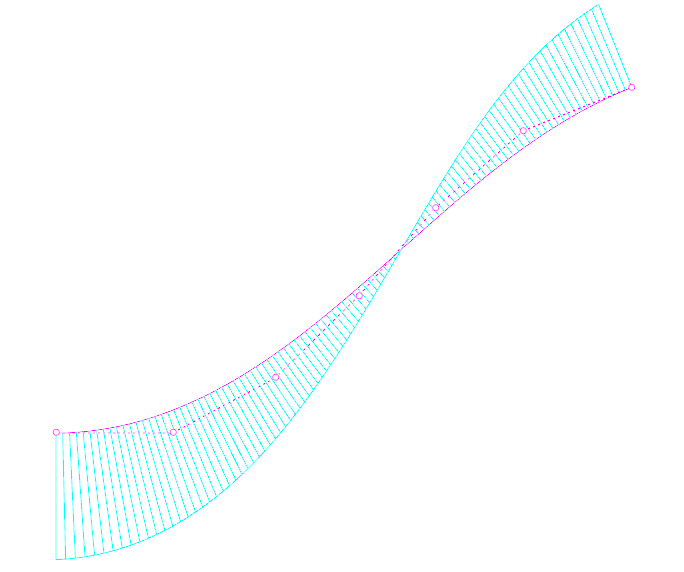
\includegraphics[width=0.9\linewidth]{figures/EulerBezierDef1.png}
			\end{minipage}
			%\qquad
			\begin{minipage}{0.49\linewidth}
				\centering
				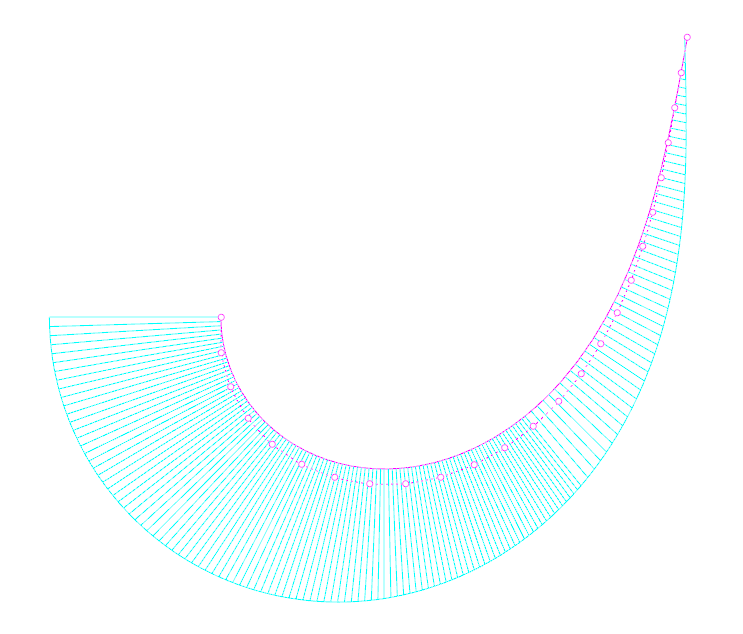
\includegraphics[width=0.9\linewidth]{figures/EulerBezierDef2.png}
			\end{minipage}
			\caption{Euler Bezier曲线}
		\end{figure}
		
		
		\section{利用Euler B\`{e}zier曲线和Euler B-Spline曲线构造G2连续圆角曲线}
		\subsection{二维Euler B\`{e}zier曲线}
		对于一个给定的多边形, 对转角做圆角处理是非常常见的需求, 传统的方法是使用圆弧, 通过确定圆弧的半径来控制圆角的程度. 由于圆弧是固定曲率的, 这种传统的方法只能构造$G^1$连续的圆角, 使用Euler B\`{e}zier曲线则可以构造出$G^2$连续的圆角曲线, 并且可以保证有且仅有一个曲率极值点.\par
		考虑多边形的一个转角$\boldsymbol{ABC}$, 我们对转角$\boldsymbol{B}$构造圆角曲线. 由于Euler B\`{e}zier螺线是曲率单调的, 而多边形的圆角曲线要达到$G^2$连续需要保证两端的曲率为0, 所以我们使用对称的两条Euler B\`{e}zier螺线拼接得到圆角曲线. 设圆角曲线的起点$\boldsymbol{P}_S$在边$\boldsymbol{AB}$上, 由于要构造对称的两条曲线, 我们把一边曲线的终点$\boldsymbol{P}_E$取在多边形的内角平分线上. 为保证$G^1$连续, 起点$\boldsymbol{P}_S$处的切方向为向量$\boldsymbol{AB}$的方向, 记为$\boldsymbol{T}_S = \boldsymbol{AB}/\Arrowvert\boldsymbol{AB}\Arrowvert$. 终点$\boldsymbol{P}_E$处的切向$\boldsymbol{T}_E$应当与多边形的内角平分线垂直. 假设Bezier曲线$\boldsymbol{P}(t)=\sum_{i=0}^n\boldsymbol{P}_iB_{i,n}(t),t\in[0,1]$插值了这两个边界条件, $\boldsymbol{P}_i\boldsymbol{P}_{i+1}$到$\boldsymbol{P}_{i+1}\boldsymbol{P}_{i+2}$的角为$\theta_{i+1}(i=0,1,\dots,n-2)$. 那么可以得到
		\begin{equation}
			\prod_{i=1}^{n-1}\text{R}(\theta_i)\boldsymbol{T}_S =  \boldsymbol{T}_E
		\end{equation}
		其中$\text{R}(\theta)$表示旋转角为$\theta$的旋转矩阵. 根据定义($\ref{EB_Def}$), $\theta_i$应当为等差数列. 考虑Bezier曲线的起点曲率$$\kappa(0)=\frac{n-1}{n}\frac{\sin(\theta_1)}{l}$$
		保证$G^2$连续要令$\kappa(0)=0$, 则有$\theta_1=0$, 故设$\theta_i=(i-1)\Delta\theta(i=1,\dots,n-1)$, 为了保证对称性, $\boldsymbol{T}_E$应当与多边形内角平分线垂直, 则$\boldsymbol{T}_S$到$\boldsymbol{T}_E$的夹角为$\alpha/2$, 所以有
		\begin{equation}
			\sum_{i=1}^{n-1}\theta_i = \frac{(n-2)(n-1)}2\Delta\theta = \frac{\alpha}2
		\end{equation}
		计算得$\Delta\theta=\frac{\alpha}{(n-2)(n-1)}$, 从而计算每个$\theta_i$. Euler多边形顶点的序列可以递推给出:
		\begin{equation}\label{recur}
			\begin{aligned}
				\boldsymbol{P}_0\boldsymbol{P}_1 &=l\boldsymbol{T}_S\\
				\boldsymbol{P}_1\boldsymbol{P}_2 &=\text{R}(\theta_1)\boldsymbol{P}_0\boldsymbol{P}_1\\
				\dots\\
				\boldsymbol{P}_i\boldsymbol{P}_{i+1} &=\text{R}(\theta_i)\boldsymbol{P}_{i-1}\boldsymbol{P}_i
			\end{aligned}
		\end{equation}
		根据起点终点条件有$\boldsymbol{P}_0=\boldsymbol{P}_S, \boldsymbol{P}_n = \boldsymbol{P}_E$, 结合递推式($\ref{recur}$)得到:
		\begin{equation}
			\boldsymbol{P}_S\boldsymbol{P}_E = \sum_{i=0}^{n-1}\boldsymbol{P}_i\boldsymbol{P}_{i+1} = l[\sum_{i=0}^{n-1}\text{R}(\phi_i)]\boldsymbol{T}_S
		\end{equation}
		其中$\phi_i=\sum_{j=1}^i\theta_j (i = 1,\dots,n-1), \phi_0 = 0$. 对于一个给定正整数$n$, 我们可以计算出向量$\boldsymbol{D} = \sum_{i=0}^{n-1}\text{R}(\phi_i)\boldsymbol{T}_S$, 这是一个常向量, 从起点到终点的连线必须与它平行. 将向量$\boldsymbol{D}$与向量$\boldsymbol{T}_S$的夹角记为$\beta$, 则有
		\begin{equation}\label{sinthoery}
			\frac{\Arrowvert\boldsymbol{OP}_S\Arrowvert}{\cos(\frac{\alpha}2-\beta)}=\frac{\Arrowvert\boldsymbol{OP}_E\Arrowvert}{\sin(\beta)}=\frac{\Arrowvert\boldsymbol{P}_S\boldsymbol{P}_E\Arrowvert}{\cos(\frac{\alpha}2)}
		\end{equation}
		根据方程$(\ref{sinthoery})$, 我们可以在给定圆角起点$\boldsymbol{P}_S$或者给定角平分线上的经过点$\boldsymbol{P}_E$时唯一求得离散的Euler螺线.
		\IncMargin{1em}
		 \begin{algorithm}
		 	\SetKwData{Left}{left}\SetKwData{This}{this}\SetKwData{Up}{up}
		 	\SetKwFunction{Union}{Union}\SetKwFunction{FindCompress}{FindCompress}
		 	\SetKwInOut{Input}{input}\SetKwInOut{Output}{output}
		 	\caption{Euler B\`{e}zier圆角}\label{smoothcurve1}
		 	\KwData{ 构成Corner的三个顶点$\boldsymbol{A},\boldsymbol{B},\boldsymbol{C}$, $\boldsymbol{BP}_S$的长度$L_S$或$\boldsymbol{BP}_E$的长度$L_E$}
		 	\KwResult{
		 	Bezier曲线$\boldsymbol{P}(t)$的控制顶点序列$\boldsymbol{P}_0,\boldsymbol{P}_1,\dots,\boldsymbol{P}_n$和对称的顶点序列}
		 	\BlankLine 
		 	 $n=4$\;
		 	 \bf{初始化B\`{e}zier曲线}$\boldsymbol{P}(t)$\;
		 	$\boldsymbol{T}_S = \text{Normalize}(\boldsymbol{B}-\boldsymbol{P}_S)$\;
		 	$\boldsymbol{D}=\boldsymbol{T}_S$\;
		 	$\boldsymbol{temp}=\boldsymbol{T}_S$\;
		 	
		 	\While{\text{EulerB\`{e}zierSpiralCheck}($\boldsymbol{P}(t)$)==\text{FALSE} and $n < 20$}{
	计算$\boldsymbol{A}\boldsymbol{B}$与$\boldsymbol{B}\boldsymbol{C}$的夹角$\alpha$\;
		 	$\Delta\theta = \frac{\alpha}{ (n - 2)  (n - 1)}$\;
		 	\For{$i=0,1,\dots,n-2$}{
		 	$\boldsymbol{temp}.\text{Rotate}(i*\Delta\theta)$\;
		 	$\boldsymbol{D}+=\boldsymbol{temp}$\;
		 }
		 	计算$\boldsymbol{A}\boldsymbol{B}$与$\boldsymbol{D}$的夹角$\beta$\;
		 	$\text{length} = \cos(\alpha / 2) / \cos(\alpha / 2 - \beta) * \Arrowvert\boldsymbol{B} - \boldsymbol{P}_S\Arrowvert / \Arrowvert \boldsymbol{D}\Arrowvert$\;
		 	$\boldsymbol{temp}=\boldsymbol{T}_S*\text{length}$\;
		 	$\boldsymbol{P}_0=\boldsymbol{P}_S$\;
		 	\For{$i=1,\dots,n-1$}{
		 	$\boldsymbol{P}_i=\boldsymbol{P}_{i-1}+\boldsymbol{temp}$\;
		 	$\boldsymbol{temp}.\text{Rotate}((i-1)*\Delta\theta)$\;
		 }
		 	$n++$\;
		 }
		 \end{algorithm}
		 \begin{figure}[htbp]
		 	\centering
		 	\begin{minipage}{0.49\linewidth}
		 		\centering
		 		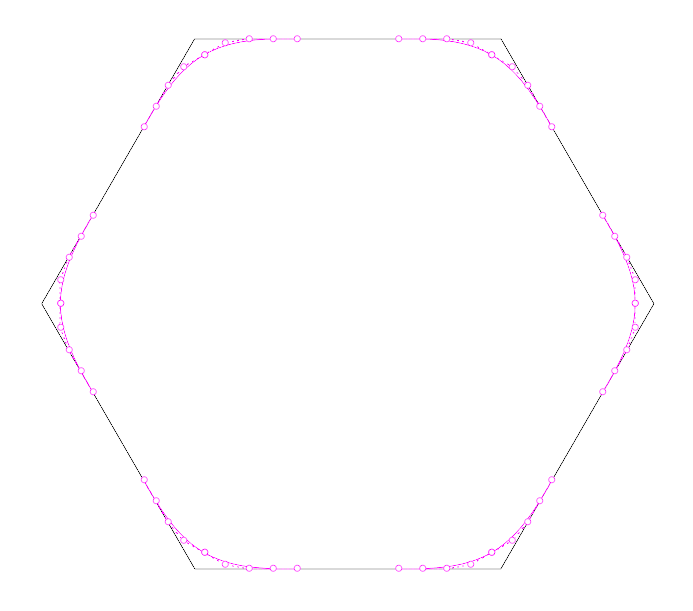
\includegraphics[width=0.9\linewidth]{figures/SmoothCorner1.png}
		 	\end{minipage}
		 	%\qquad
		 	\begin{minipage}{0.49\linewidth}
		 		\centering
		 		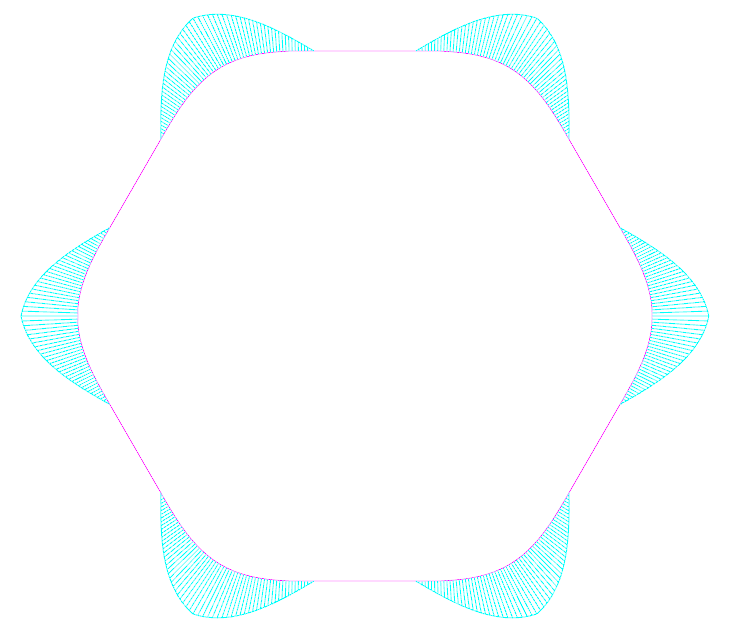
\includegraphics[width=0.9\linewidth]{figures/SmoothCorner2.png}
		 	\end{minipage}
		 	\caption{算法($\ref{smoothcurve1}$)得到的$G^2$连续Euler B\`{e}zier螺线圆角}
		 \end{figure}
	 \subsection{二维Euler B-Spline曲线}
	 \section{三维Euler B\`{e}zier 曲线与Euler B-Spline 曲线}
	 \subsection{二维到三维的方法}
	 三维空间中插值$G^1$边界条件的曲率(以及挠率)单调曲线的存在性不像二维的情形有简单且完整的理论证明
	 \subsection{三维Euler B\`{e}zier 曲线}
	 \subsection{三维Euler B-Spline 曲线}
		
		
		\renewcommand\refname{参考文献}
		\addcontentsline{toc}{section}{参考文献}
		\begin{thebibliography}{100}%此处数字为最多可添加的参考文献数量
				\bibitem{article1}第一篇文献.
				\bibitem{article2}第二篇文献.
				\bibitem{article3}第三篇文献.
				\bibitem{article4}第四篇文献.
		\end{thebibliography}  
\end{document}